\documentclass[twoside,b5paper,10pt]{article}
\usepackage{AUTstyle}

\usepackage{hyperref}
\usepackage[]{mcode}
\lstdefinestyle{customc}{
  belowcaptionskip=1\baselineskip,
  breaklines=true,
  frame=L,
  xleftmargin=\parindent,
  language=C,
  showstringspaces=false,
  basicstyle=\footnotesize\ttfamily,
  keywordstyle=\bfseries\color{green},
  commentstyle=\itshape\color{green},
  identifierstyle=\color{black},
  stringstyle=\color{orange},
}

\title{Development of an Autonomous Ground Vehicle for the RobonAUT 2014 Contest}
\author{Csorvási Gábor \and Fodor Attila}

\institution{Department of Automation and Applied Informatics \\
Budapest University of Technology and Economics}

\email{\{csorvagep, attila.fodor.89\}@gmail.com}

\headerTitle{Development of an AGV\dots}
\headerAuthor{Csorvási Gábor and Fodor Attila}

% Style Guide:
% Technologies: Enclose them with \verb!name! e.g.: \verb!MATLAB!
% Important anocryms, titles, etc: Enclose them in \textbf{name} to get bold typeface. e.g. \textbf{RobonAUT}
% Emphasis: Enclose in \emph{name}

\begin{document}
\makeAutStyleTitle


\begin{abstract}
RobonAUT is a local robot development contest of the Faculty of Electrical Engineering and Informatics of BME. This paper describes the development process of an Autonomous Ground Vehicle which was one of the successful competitors of the 2014 contest. During software development of the embedded control system the possibilities of rapid prototyping have been exploited extensively. The paper demonstrates the power of model based design of control systems and embedded software, and describes the rapid deployment method in detail, which was used to integrate the MATLAB model with FreeRTOS on the target hardware.
\end{abstract}


\begin{keywords}
RobonAUT; Autonomous; AACS Workhsop; MATLAB; Real-Time; Control Systems; ...
\end{keywords}

\section{Bevezetés}

A dokumentum abból a célból jött létre, hogy segítséget nyújtson \verb!STM32F4-Discovery! board alapú projektek fejlesztéséhez. A szükséges lépések nagyrészét igyekszünk bemutatni valós alkalmazások segítségével, melyeknek túlnyomó többsége a 2014-es \textbf{RobonAUT} versenyre történő felkészülés közben került kivitelezésre. A problémák számunkra is újak voltak, így nem ígérhetjük, hogy a legjobb megoldásokat fogjuk prezentálni itt, de a bemutatott eljárásról kijelenthetjük, hogy hasznosnak és megbízhatónak bizonyult.

Az írást három fő részre osztottuk, először bemutatásra kerülnek a \verb!MATLAB-Simulink! modell alapú tervezés lépései és a fordítható kód generálása. Ezután a generált kód integrálására és élesztésére térünk rá \verb!FreeRTOS! operációs rendszer alatt, legvégül pedig valós gyors prototípustervezési technikák kerülnek bemutatásra, a \verb!MATLAB! közvetlen \verb!STM32F4-Discovery! hardware támogatását felhasználva.

\begin{figure}[!ht]
    \centering
    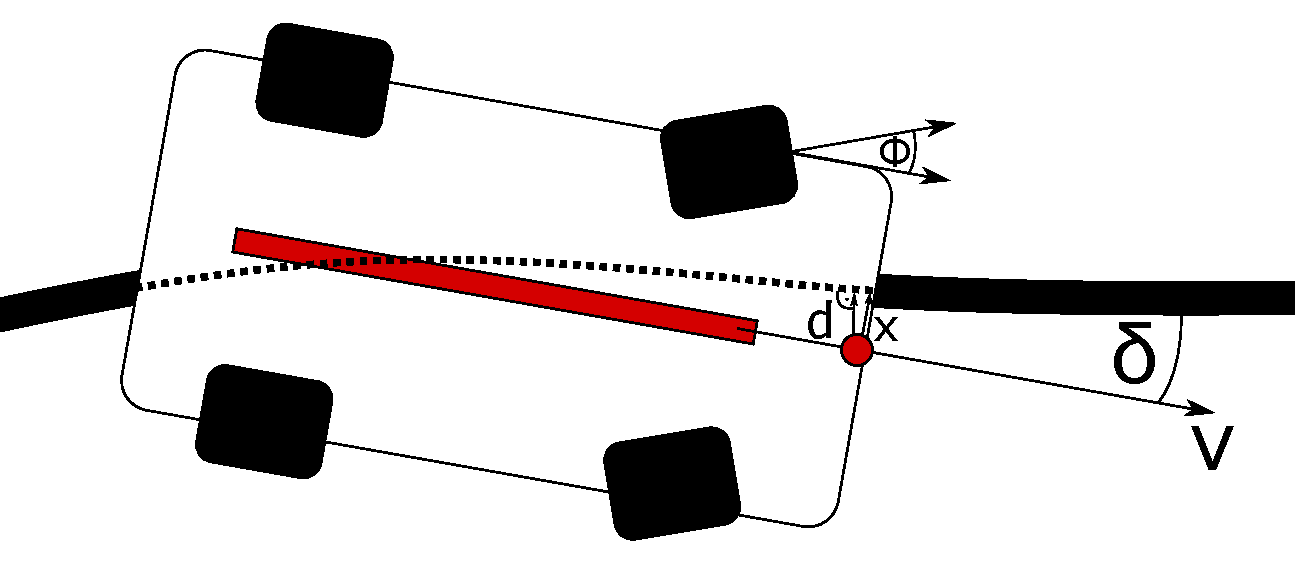
\includegraphics[width=0.9\linewidth]{img/cartop}
    \caption{A probléma sematikus ábrája felülnézetből}
    \label{fig:cartop}
\end{figure}

A \textbf{RobonAUT} verseny során egy olyan robot szoftverét és hardverét kell elkészíteni, amely lehetővé teszi a távirányítós autóból átalakított platformot, hogy egy ismeretlen pályán végighaladjon, és ott akadályokat teljesítsen, a szabályzatban meghatározott módon. A továbbiakban csak a szoftver környezettel foglalkozunk és feltételezzük, hogy megfelelő logikai jelek zajjal terhelten bár, de rendelkezésre állnak a szenzorokból, illetve az autó várakozásainknak megfelelően reagál a kimeneti jelekre, pl. a kormányszög beállítására.

A dokumentumban próbáljuk a szakirodalomban elterjedt jelrendszert alkalmazni, de az alábbi táblázat segítségével magyarázzuk a rendszeresen előforduló jelöléseket és összefüggéseket. Amennyiben valami hiányzik innen, az a szövegkörnyezetben kerül definiálásra.

\begin{center}
  \begin{tabular}{| c | p{0.8\linewidth} |}
\hline
    d & Pozícióhiba: Az első optikai szenzorsor középpontjának távolsága a vonaltól \\ \hline
    $ \delta $ & Szöghiba: Az első optikai szenzorsorra merőleges egyenes (középvonal) és a pályavonal érintője által bezárt szög \\ \hline
    $ \Phi $ & Kormányszög: A kerekek síkjainak a középvonallal bezárt szögeinek átlaga, Ackermann-kormányzás szerint \\
    \hline
    $ \kappa $ & A pálya pillanatnyi görbülete ($1/R$) \\ \hline
    x & Vonalpozíció: az első optikai szenzorsor által érzékelt vonalak középpontjának előjeles távolsága a szenzorsoron a közepponttól mérve. \\ \hline
    c & Vonalsebesség: x első deriváltja, a vonalpozíció mozgásának sebessége \\ \hline
    v & Sebesség: Az autó pillanatnyi sebessége a középvonal mentén \\
    \hline
  \end{tabular}
\end{center}
\section{Integration}
\label{sec:integration}

\subsection{Structure of the code}

If during the code generation \emph{Compact code placement} was used, only four files are generated:

\begin{itemize}

    \item "system\_name".c
    \item "system\_name".h
    \item rtwtypes.h
    \item ert\_main.c

\end{itemize}

In the following we assume that the name of the Controller block was "controlsystem".

\begin{figure}[!ht]
    \centering
    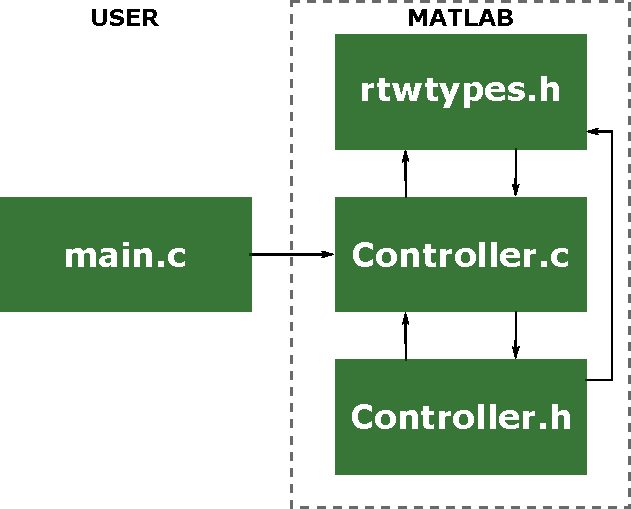
\includegraphics[width=0.6\linewidth]{img/rtw}
    \caption{Relationship of the generated files}
    \label{fig:rtw}
\end{figure}

The functions of the system are defined in the \textbf{controlsystem.c} and \textbf{controlsystem.h} files. The \textbf{rtwtypes.h} contains the unique type definitions of the code. The \textbf{ert\_main.c} is an exemplary main function that demonstrates the use of the others.

\subsection{Using the code}

The generated source code is functionally a perfect equivalent of the \verb!Simulink! model. The system can be initialized using the \emph{controlsystem\_initialize()} function. It sets the 0 time in the model and the outputs obtain their initial values. Communication with the system is only possible through a unique interface provided by the generated code. The inputs are handled by the \emph{controlsystem\_U struct}. It contains fields each corresponding to a system input, matching it's name and type. If the inputs are set, calling the \emph{controlsystem\_step()} function runs the model once, for the period of one time sample. The outputs are stored in a structure similar to the input storage, called \emph{controlsystem\_Y}.

\subsection{Deployment with FreeRTOS on STM32F4-Discovery Board}

As in many controlled processes, the timing of the controller program execution is crucial. Beside that it is also a time crucial task to process the I/O lines, convert the analog signals, and send status information to the supervisor computer over a wireless connection. It can be done with the integrated timer peripherals and with interrupt sequences, but the easiest way to handle a multi task problem like ours, is a \textbf{Real Time Operating System}. There are numerous implementation of these operating systems. We chose the FreeRTOS, which is a well known operating system in the industry, open-source, well documented and last but not least we have experience with it.

In our solution the FreeRTOS is responsible for the task scheduling, and provide a communication interface between the tasks. This way we can ensure that the sensors are read in the appropriate time, and the controller task will run in the specified time period. Also provides some useful tools to debug the application.
%Freertos mint Core mit csinál? (beszélget a hardverrel, szenzorokkal, aktuárotoknak küld beavatkozó jeleket)
%Miért jó? (gyors hozzáférés a szenzorokhoz, pontos ütemezés a controllernek)

Setting up the system is quite easy in this point. We only have to include the FreeRTOS source files into our project.\footnote{A detailed description is available for many processors in the FreeRTOS website: http://www.freertos.org/} The next step is to write some low level driver to read the sensors, and initialize the actuators so this way we can connect these to the control system. It is also necessary to set up the communication between the tasks, so we can read the state of the controller and the other tasks real time.
%Mit kellett csinálni, hogy működjön? (FreeRTOS-t feltenni rá (max 1 mondat, ebbe nem megyünk bele!), hardver jeleket kiolvasni C-vel, hogy oda tudjuk adni a controllernek, matlab-ot rákötni egy interrupt-ra)
%Még mit kell csinálni, hogy működjön?? Max 1-2 mondat már csak.
\section{Hardware-támogatás}

A MATLAB 2013b verziójától elérhető direkt hardware-támogatás az STM32F4 Discovery fejlesztőkártyához, melyet a MATLAB Hardware Support oldaláról tölthetünk le. A támogatás segítségével villámgyorsan tesztelhetjük az elkészített szoftvert, soros kábel segítségével pedig akár Processor-in-the-Loop tesztet is végrehajthatunk\cite[]{pilveri}.

\subsection{Gyors Prototípustervezés}

A RobonAUT elsősorban gyors prototípustervezési munkát igényel. Rövid idő alatt, minél hatékonyabb párhuzamosítással és a lehető legkevesebb teszteléssel kell sok funkcióval rendelkező, többé-kevésbé megbízható rendszert építeni. A magas és az alacsony szintű irányítás fejlesztése teljesen párhuzamosan zajlik, ha megfelelően kiaknázzuk a lehetőségeket.

\paragraph{Példa} Készítsünk Simulinkben egy LED-villogtató programot 5 perc alatt!

Miután feltelepítettük a support package-et\footnote{Ekkor indul a stopper}, hozzunk létre egy új Simulink modellt, majd húzzuk be az \textbf{Embedded Coder Support Package for STMF4-Discovery Board} library-ből a szükséges blokkokat. Az ábrán látható módon állítuk össze a kapcsolást, majd konfiguráljuk a modellt az 1. részben leírtakhoz hasonlóan, de most a \textbf{Code Generation} menüben \textbf{Target Hardware}-nek válasszuk az \verb!STM32F4-Discovery!-t, valamint ne csak kódot generáljunk (Pipa ki a \textbf{Generate code only} checkbox-ból).\footnote{Cheat sheet újoncoknak: A \texttt{Constant} blokk signal type-ját  \texttt{boolean}-re, a  \texttt{Pulse Generator} Pulse type-ját pedig  \texttt{Sample based}-re kell állítani. A blokkokról pedig senki sem tudja, hogy melyik almenüben vannak, érdemes használni a keresőt. Ne felejtsük el a GPIO blokkok konfigurálását sem! Ha semmiképpen sem akar működni, akkor a kész modell letölthető \href{http://www.mathworks.com/matlabcentral/fileexchange/45953-stm32f4-discovery-led-blinker}{\texttt{innen}}.}

\begin{figure}[!ht]
    \centering
    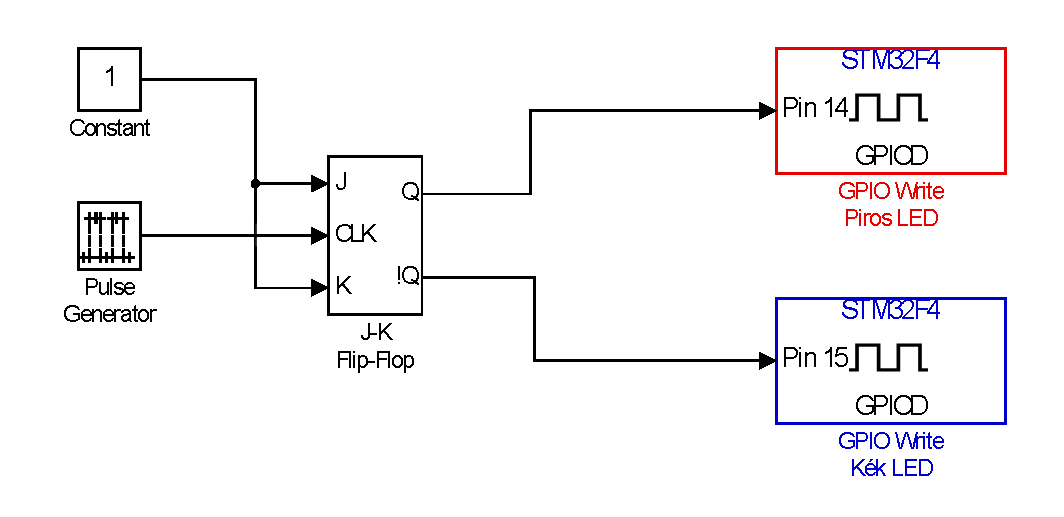
\includegraphics[width=0.9\linewidth]{img/stmblink}
    \caption{LED villogtató Simulink-modell}
    \label{fig:stmblink}
\end{figure}

A teljes rendszert a \textbf{Code} menü \textbf{C/C++ Code} menüpontjából tudjuk buildelni. Ha mindent jól csináltunk, a jutalmunk a végén egy \verb!.hex!, egy \verb!.elf! és egy \verb!.bin! file lesz a Working Directory-ben. Ezután az \texttt{STM ST-LINK Utility} segítségével felprogramozhatjuk a kártyát a generált fileok segítségével. Természetesen nem csak a ledeket tudjuk villogtatni, hanem az összes GPIO-t, gombot és analóg I/O-t kezelni tudjuk tetszőlegesen bonyolult modell köré építve. A GPIO Read és Write blokkok beállításához az \texttt{ST-Microelectronics} megfelelő segédletet nyújt\cite{usermanual}.

Hasonló elv alapján épült fel egy standard servo jeleket feldolgozó projekt is, melyet egy távirányítós autó végfokozatának PWM-es vezérlésére használtam.A Simulink modell szintén letölthető \href{http://www.mathworks.com/matlabcentral/fileexchange/46221-rc-car-control-with-stm32f4-discovery-programmed-by-matlab}{\texttt{innen}}, és mélyebb betekintést ad a modell alapú tervezés nyújtotta lehetőségekbe. Egy ilyen feladat elkészítése is inkább munkapercekben, mint -órákban mérhető.
Korábban említettük, hogy akár PIL tesztelésre is lehetőség van. Ebben a dokumentumban erre az alkalmazási területre nem térünk ki, de egy későbbi bővített kiadásban előfordulhat, ha igény mutatkozik a témára.
\section{Results and future work}

The most important result is the successful application of the method. The system was designed and implemented in \verb!MATLAB!-generated code embedded into a \verb!FreeRTOS! Core, based on the methods described in this paper. Despite the odds and a challenging competition during the RobonAUT 2014, our car have scored a podium finish. It demonstrated complete reliability, though there have been performance issues in the faster sections, due to a flaw in the controller design. We plan to participate in the RobonAUT 2015 competition as well, and utilize the direct hardware support of \verb!MATLAB! for the \verb!STM32F4-Discovery!.

\section{Conclusion}



\section*{Acknowledgments}
 { \small The author would like to express his thanks to István Vajk~\footnote{Please mention the name of your advisor in the
Acknowledgements section. } for his support as a scientific advisor.
This work has been supported by the \dots \footnote{Please mention
the institution or organization that has supported your research
work.} }

% NOTE!
% When changing the BiBTeX file, the following procedure must be followed to obtain a document with working references:
% Compile PDF LaTeX
% Compile BiBTeX
% Compile PDF LaTeX
% Compile PDF LaTeX
% Now check the output
\makeAutBib{bibs}

\end{document}
